\section{The identification boundary}\label{sec:ident}

A central question in algorithmic market surveillance is whether an observer of executions and prices can identify the individual strategies active in the market.

\begin{theorem}[Merged rate--weight equivalence]\label{thm:merged}
Let $\kappa>0$ and $a\in[0,1)$ be known. Use zero initial states and a common probe contract, and observe the modeled price state $x_t$.
\begin{enumerate}[label=(\roman*)]
\item \emph{Equivalence class.} Two economies $\mathcal E^A=\{(q_i^A,\eta_i^A)\}$ and $\mathcal E^B=\{(q_j^B,\eta_j^B)\}$ produce identical price responses for every probe sequence if and only if their merged measures coincide:
\begin{equation}\label{eq:merged}
\sum_{i:\eta_i^A=\eta} q_i^A\eta \;=\; \sum_{j:\eta_j^B=\eta} q_j^B\eta\qquad\forall\eta\in(0,1).
\end{equation}
The minimal realization has dimension $1+|\mathrm{supp}(M)|$, counting distinct rates with nonzero merged weight after signed cancellation. A cohort with $\eta=1$ merges into the anchor $a$ without adding a pole.
\item \emph{Separation complexity under average power.} Consider testing a single cohort with rate $\bar\eta$ against two cohorts with rates $\bar\eta\pm\delta$ and the same total weight, on a compact family that is uniformly Schur stable with rates bounded away from $0$ and $1$. Observe $\tilde x_t=x_t+\nu_t$ with $\nu_t\sim N(0,\sigma_\nu^2)$ and use deterministic probes with $\frac1T\sum_{t<T}v_t^2\le P$. Any test with worst-case error at most $\alpha\in(0,1/4)$ needs
\begin{equation}\label{eq:Tpower}
T\;\ge\;\frac{4\sigma_\nu^2(1-2\alpha)^2}{K^2P\,\delta^4}=\Omega(\delta^{-4}),
\end{equation}
where $K$ depends only on the family.
\end{enumerate}
\end{theorem}

The memory rates are poles of $G$ and \emph{zeros} of $H$, not closed-loop poles. This has a practical consequence we verify in Section~\ref{sec:mixtures}: pole-fitting methods applied directly to the price impulse response recover closed-loop eigenvalues ($0.4256$ and $0.8224$ for $K=1$, $\eta=0.3$, $a=0.5$, $\kappa=0.8$, $q=0.2$) and miss the memory rate $0.70$.

\begin{remark}[Scope]\label{rem:scope}
The result concerns the stated model and observation contract. Cohorts sharing an exact rate enter prices through their merged weight; this does not determine identities or wealth allocations. Nearby rates can be distinguishable with enough information. The $\delta^{-4}$ statement in (ii) is a lower bound on a declared family, with family-dependent constants. Individual algorithms may choose their rates strategically, but any unilateral change maps into the same observer-facing merged measure, which reinforces rather than circumvents the boundary.
\end{remark}

\section{Probing resources, memory resolution and money}\label{sec:resources}

Observation length alone cannot buy identification when the lifetime quantity of controlled executions is fixed. This section connects the merged-memory experiment to a financially specified input/output contract. Throughout, $\Phi$ is the standard normal distribution function.

\subsection{Quantity}

\begin{theorem}[Sharp probing-resource orders for a known symmetric pair]\label{thm:quantity}
Fix $0\le a<1$, $\kappa,q>0$, $S=a+\kappa q<1$ and $\eta\in(0,1)$. Compare a single cohort of weight $q$ and rate $\eta$ with two cohorts of weight $q/2$ and rates $\eta\pm\delta$, both in $[\epsilon,1-\epsilon]$. All parameters are known. The price receives executed quantity through $\kappa v_t$, starts from zero, has no process noise, and is observed with independent $N(0,\sigma^2)$ noise. Probes are deterministic and common to both alternatives. Let $d_T=(h^\delta_j-h^0_j)_{j<T}$ and $K_*=2\kappa^2q/[\epsilon^3(1-S)^2]$.
\begin{enumerate}[label=(\roman*)]
\item For every probe with $\sum_t|v_t|\le V$,
\begin{equation}\label{eq:klV}
\KL(P_0^v\|P_\delta^v)\le\frac{K_*^2V^2\delta^4}{2\sigma^2},\qquad e_{\rm worst}\ge\frac12\Bigl(1-\frac{K_*V\delta^2}{2\sigma}\Bigr)_+ .
\end{equation}
\item The optimal worst-case error over these probes and all classifiers is exactly
\begin{equation}\label{eq:exacterr}
e^*_T(V)=\Phi\!\left(-\frac{V\|d_T\|_2}{2\sigma}\right),
\end{equation}
attained by a pulse at the first input and the likelihood-ratio test. Waiting adds information but $\|d_T\|_2\uparrow\|d_\infty\|_2<\infty$, so it cannot make the error arbitrarily small at fixed $V$. Error at most $\alpha<1/2$ requires $V\ge2\sigma(1-2\alpha)/(K_*\delta^2)$ independently of $T$.
\item The first two taps coincide and $d_2=-\kappa^2q\delta^2$. A single pulse of size
\begin{equation}\label{eq:pulse}
A=\frac{2\sigma\Phi^{-1}(1-\alpha)}{\kappa^2q\delta^2}
\end{equation}
and the third observation achieve error exactly $\alpha$. The necessary and sufficient quantity order is $\delta^{-2}$.
\item Under average power $\sum_{t<T}v_t^2\le PT$, the necessary horizon order is $\delta^{-4}$, attained by the pulse whenever $T\ge\max\{3,\lceil A^2/P\rceil\}$.
\item For a fixed monetary price exposure $\lambda\neq0$, additive reserve $L$ and cost envelope $c\sum|v_t|$, the sharp robust quantity allowance under budget $B>L$ is $V_B=(B-L)/(|\lambda|\kappa+c)$.
\end{enumerate}
\end{theorem}

The identity in (iii) is verified to machine precision for $\delta\in\{0.02,0.05,0.10\}$: the difference is $-1.2\times10^{-4}$, $-7.5\times10^{-4}$ and $-3.0\times10^{-3}$ at $\kappa=1$, $q=0.3$, and $-3.2\times10^{-4}$ at the calibration $\kappa=0.8$, $q=0.2$, $\delta=0.05$. The theorem does not solve estimation of an unknown mixture (Section~\ref{sec:mixtures}).

\begin{figure}[t]\centering
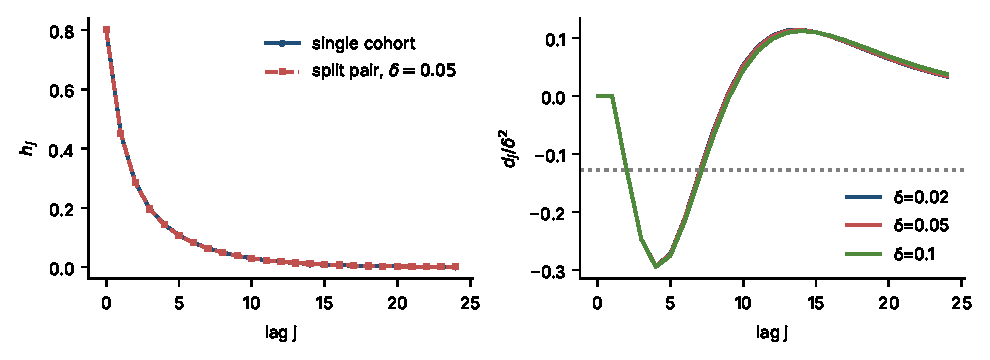
\includegraphics[width=\textwidth]{figs/fig_impulse.pdf}
\caption{Left: impulse responses of the single cohort and the split pair ($\delta=0.05$) are nearly indistinguishable. Right: the difference scaled by $\delta^2$ collapses onto one curve, with first nonzero value $-\kappa^2q$ at lag 2 (dotted). Calibration $a=0.5$, $\kappa=0.8$, $q=0.2$, $\eta=0.4$.}\label{fig:impulse}
\end{figure}

\paragraph{A Monte Carlo check of the exact error.} Formula \eqref{eq:exacterr} is exact for the likelihood-ratio test. We simulated 200,000 noisy paths per hypothesis at the calibration ($\sigma=0.01$, $\delta=0.05$) for several pulse sizes and horizons (Table~\ref{tab:mcerr}); simulated errors match the formula to Monte Carlo precision under both hypotheses.

\begin{table}[t]\centering
\begin{threeparttable}
\caption{Exact known-pair error: formula versus simulation}\label{tab:mcerr}
\begin{tabular}{rrccc}
\toprule
Pulse $V$ & Horizon $T$ & $\Phi(-V\|d_T\|_2/2\sigma)$ & Simulated error, $H_0$ & Simulated error, $H_\delta$\\
\midrule
20 & 3 & 0.3745 & 0.3734 & 0.3762\\
40 & 3 & 0.2611 & 0.2599 & 0.2603\\
40 & 10 & 0.0029 & 0.0030 & 0.0027\\
80 & 20 & $1.8\times10^{-10}$ & 0 & 0\\
\bottomrule
\end{tabular}
\begin{tablenotes}\footnotesize\item 200,000 paths per hypothesis; $a=0.5$, $\kappa=0.8$, $q=0.2$, $\eta=0.4$. \end{tablenotes}
\end{threeparttable}
\end{table}

Figure~\ref{fig:impulse} shows why the problem is hard. The two economies have the same direct impact and the same first-lag response; they first differ at lag two, by an amount proportional to $\delta^2$, and the whole difference sequence scales with $\delta^2$. A test therefore needs the signal-to-noise ratio $V\|d\|/\sigma$ to grow like $\delta^{-2}$, which is the quantity order, and because the adverse mark of a probe grows with the square of its size, capital grows like $\delta^{-4}$.

\subsection{Execution cost}

A probe changes inventory as well as price. We therefore specify cash and execution timing. Price has units of currency per asset, and $\kappa$ currency per squared quantity.

\begin{lemma}[Fair execution]\label{lem:toeplitz}
For a quote schedule refreshed after the uncontrolled state update, execution at the average price of a linear book costs, relative to the constant fundamental mark,
\begin{equation}\label{eq:cost}
C(v)=\tfrac12v^\top T_hv+c\|v\|_1,\qquad (T_h)_{ij}=h_{|i-j|}.
\end{equation}
In the positive stable economy $T_h$ is positive definite, so no nonzero round trip produces a deterministic gain.
\end{lemma}

We verify the ledger identity \eqref{eq:cost} against an explicit cash account to $5.7\times10^{-13}$ on 1,000 random probes, and the smallest eigenvalue of $T_h$ over 1,000 random stable positive economies is $0.141$. A direct-only proxy $\sum\tfrac12\kappa v_t^2$ omits cross-time impact: for $v=(+1,-1)$ it gives $0.80$ against a true Toeplitz loss of $h_0-h_1=0.3488$.

\subsection{Capital supplied by a counterparty}

\begin{theorem}[Sharp robust quantity cap from cash and margin]\label{thm:cap}
Use the positive, stable, reset economy with constant fundamental price $P_*>0$ and no process noise. A designated dealer fills only nonnegative probes $v_t\ge0$ at the average price $P^0_{t+1}+\kappa v_t/2$ of a linear schedule, holds inventory $I_{t+1}=I_t-v_t$ and cash $K_{t+1}=K_t+v_t(P^0_{t+1}+\kappa v_t/2)-cv_t$, starts with equity $B>0$, and must satisfy $\mu|I_t|P_t\le E_t$ at every time. For the robust contract admitting every probe with $\sum_tv_t\le V$, the largest allowance guaranteeing margin is
\begin{equation}\label{eq:VB}
V_B=\frac{2B}{\beta+\sqrt{\beta^2+4(\mu+\tfrac12)\kappa B}},\qquad\beta=c+\mu P_*,
\end{equation}
equivalently $(\mu+\tfrac12)\kappa V^2+(c+\mu P_*)V\le B$. The cap holds across all positive cohort representations with $S<1$, without resolving individual rates. An observer that receives only noisy prices and executed quantities has best error $\Phi[-V_B\|d_T\|_2/(2\sigma)]$ within this allowance; fixed error $\alpha<1/2$ requires capital of order at least $\delta^{-4}$, and a single positive pulse attains that order.
\end{theorem}

Even with zero initial inventory, the probe creates a quadratic adverse mark that a fixed initial price exposure would miss. Figure~\ref{fig:knownpair} illustrates the experiment.

\begin{figure}[t]\centering
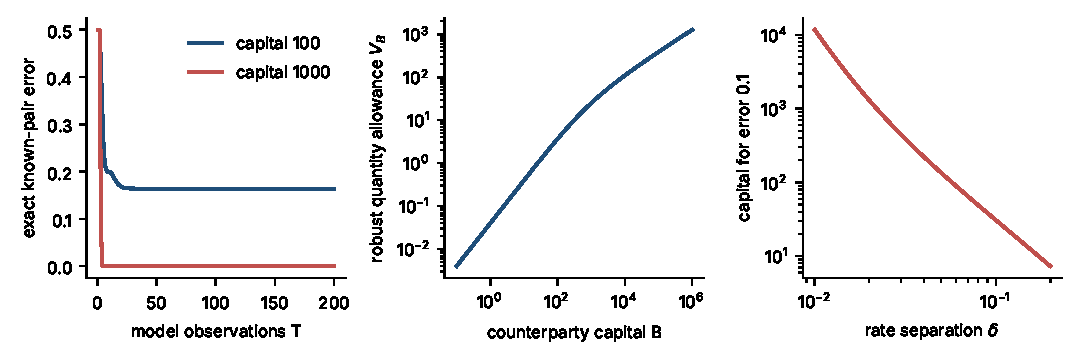
\includegraphics[width=\textwidth]{figs/fig_knownpair.pdf}
\caption{Known-pair experiment funded by the counterparty cash/margin contract. (a) Exact Gaussian error at fixed capital 100 and 1,000, separation $\delta=0.05$. (b) The sharp robust quantity allowance \eqref{eq:VB}. (c) Capital for error $0.1$ with 200 observations. Parameters: $a=0.5$, $\kappa=0.8$, $q=0.2$, $\eta=0.4$, observation s.d.\ $0.003$, reference price 100, margin $0.25$, cost $0.02$. No process noise.}\label{fig:knownpair}
\end{figure}

\begin{proposition}[Exact financial disclosure changes the experiment]\label{prop:disclosure}
In this noiseless-state account, exact disclosure of the third equity mark after a single positive pulse $0<A\le V_B$ distinguishes the known pair with zero error for every $\delta>0$.
\end{proposition}

Exact marked equity is extra information, not a free observation assumed by the price-only theorem. Real account marks have their own precision: with reports rounded to $0.01$, a guaranteed change requires a larger trade (Section~\ref{sec:disclosure}).

\subsection{Capital paid by the probe trader}

\begin{theorem}[Matching capital order for funded deterministic probes]\label{thm:capital}
Use the same economy and execution law. The statistical observer receives only noisy prices and executed quantities. The probe trader starts with cash $B>0$ and zero inventory; a finite signed sequence $v$ changes inventory by $+v_t$ and cash by $K_{t+1}=K_t-v_t(P^0_{t+1}+\kappa v_t/2)-c|v_t|$, after which trading stops and the trader must remain solvent as the price returns to $P_*$. Put
\[
r=1-\epsilon(1-S)<1,\qquad m=\kappa\frac{1-r}{1+r}>0,\qquad K_*=\frac{2\kappa^2q}{\epsilon^3(1-S)^2}.
\]
Every solvent strategy satisfies $\KL(P_0^v\|P_\delta^v)\le K_*^2B\delta^4/(\sigma^2m)$, so error at most $\alpha<1/2$ requires
\begin{equation}\label{eq:Bmin}
B\;\ge\;\frac{2\sigma^2m(1-2\alpha)^2}{K_*^2\delta^4},
\end{equation}
without a quantity cap and at any horizon. Conversely, for any margin fraction $0<\mu\le1$, the pulse $A$ in \eqref{eq:pulse} achieves error $\alpha$ and remains margin-solvent at every later mark with capital $B_A=\tfrac{\kappa}{2}A^2+(c+\mu P_*)A$. Necessary and sufficient capital orders are $\delta^{-4}$.
\end{theorem}

Theorem~\ref{thm:capital} is an order statement: an elementary time-domain coercivity argument for Toeplitz forms that establishes the $\delta^{-4}$ rate before the exact frequency-domain optimization of Section~\ref{sec:account}. Its explicit lower constant is correspondingly loose: at the calibrated parameters it evaluates to $4.9\times10^{-4}$ par units at $\delta=0.05$ with $\epsilon=0.35$, five orders of magnitude below any design we can execute. Section~\ref{sec:account} computes the constant that matters.

\subsection{A worked example: two Kalman desks}\label{sec:worked}

To make the orders concrete, consider two desks that track the same trend with Kalman filters (Proposition~\ref{prop:kalman}) and differ only in their signal-to-noise ratios: $\sigma_\zeta^2/\sigma_\nu^2=0.09$ and $0.16$. Their gains are $\eta_1=0.2584$ and $\eta_2=0.3279$, so $\bar\eta=0.2931$ and $\delta=0.0348$. With equal weights, the economy is observationally the split pair of Theorem~\ref{thm:quantity} around $\bar\eta$, and the response difference first appears at lag two, $d_2=-\kappa^2q\delta^2=-1.55\times10^{-4}$ (verified).

A supervisor who wants to tell this market from a single desk with gain $\bar\eta$ at 5\% error using a single pulse and the third observation needs $A=2\sigma\Phi^{-1}(0.95)/(\kappa^2q\delta^2)=212$ units of executed quantity, and, under a 0.5\% margin and 4 basis points of fees, single-pulse capital of $18{,}166$ par units. The pulse is very inefficient: by the $\delta^{-4}$ scaling of Theorem~\ref{thm:spectral}, the optimal flat probe needs about $61.41\times(0.05/0.0348)^4\approx262$ par units. Converting with the measured Roll noise (factor $(0.40/0.01)^2$), the optimal probe costs roughly $4\times10^5$ USDT and the naive pulse about $3\times10^7$ USDT. Two desks whose signal-to-noise ratios differ by almost a factor of two are therefore expensive, but not impossible, to tell apart by probing; three or more desks are much harder (Theorem~\ref{thm:kcohort}).

\subsection{Natural excitation and the cost of ambiguity}

\begin{proposition}[Passive distinction with zero controlled quantity]\label{prop:passive0}
Keep the known pair, but add independent uniform innovations $w_t\in[-b,b]$ of variance $s_w^2=b^2/3$ at each price update, observe $\tilde x_t=x_t+\nu_t$ with $\nu_t\sim N(0,\sigma^2)$, use independent three-step reset blocks and no probes, with $P_*>3b$. Let $b_1=a+\kappa q\eta$, $b_{2,0}=b_1^2+\kappa q\eta(1-\eta)$ and $b_{2,\delta}=b_{2,0}-\kappa q\delta^2$. In each block the covariance of the first and third observations differs by $\Delta=\kappa qs_w^2\delta^2$. With
\[
R=\max_{r\in\{0,\delta\}}\Bigl\{(s_w^2+\sigma^2)\bigl[s_w^2(1+b_1^2+b_{2,r}^2)+\sigma^2\bigr]+s_w^4b_{2,r}^2\Bigr\},
\]
the midpoint test of the average product has worst-case error at most $\alpha$ whenever $n\ge4R/(\alpha\Delta^2)$ blocks are observed: zero controlled quantity and order $\delta^{-4}$ blocks.
\end{proposition}

The Chebyshev bound is conservative but the order is real. With $b=0.03$, observation s.d.\ $0.01$ and $\delta=0.10$, the bound asks for $3.9\times10^7$ blocks at $\alpha=0.1$; in simulation the midpoint test still errs 32--38\% of the time with $2\times10^5$ blocks. Independent resets and known innovation laws are extra conditions. The proposition does not show that anonymous public records identify participants; it shows that passive excitation can accumulate memory information while the probe account stays untouched.

\begin{proposition}[Conditional quote and allocation cost of ambiguity]\label{prop:ambiguity}
Consider a one-unit ticket with adverse mark $Z_\theta\sim N(\mu_\theta,\sigma_\theta^2)$ and a CARA dealer with risk aversion $\gamma>0$. Let $c_\theta=\mu_\theta+\gamma\sigma_\theta^2/2\ge0$ with $\sup_\theta c_\theta<\infty$. Under competition with zero robust certainty equivalent, the informed quote is $s_1=c_{\theta_0}$ and the ambiguous quote $s_2=\sup_\theta c_\theta$, so $\Delta=s_2-s_1\ge0$, strictly when the worst relevant cost exceeds $c_{\theta_0}$. Under inverse demand $v(V)=(V_0-V)/b$ and marginal cost $c$, raising an interior quote from $s_0$ to $s_0+\Delta$ lowers surplus by $W_{\rm loss}=b(s_0-c)\Delta+\tfrac b2\Delta^2$.
\end{proposition}

Cohort non-identification alone does not establish that the worst relevant cost exceeds $c_{\theta_0}$; the set of relevant costs is an additional primitive. Treating a risk charge as a social cost requires a defended welfare criterion.
